\section{Analisi FEM}
A seguito dell'esito positivo delle verifiche preliminari si è proceduto alla modellazione tridimensionale dei componenti costituenti il bozzello con gancio tramite il software \textit{SolidWorks}.
La seconda fase di verifica strutturale perevede il calcolo agli elementi finiti tramite il solver \textit{Simulation} integrato in SolidWorks. 
Si parte dallo studio del sistema complessivo per analizzare la deformata della struttura e per individuare le criticità del sistema per poi concentrarsi sull'analisi dei singoli componenti. 

La prima analisi viene portata a termine su una mesh grezza, in questo modo si valuta la coerenza dei risultati. Risultati non coerenti possono emergere da un'errata configurazione di vincoli e carichi. Le successive simulazioni si effettuano su mesh che vengono via via infittite nei punti di interesse, si diagramma infine il grafico di convergenza per verificare che lo sforzo calcolato converga ad un valore preciso. 

Nella verifica è stato utilizzato un acciaio AISI 1020 presente nella libreria materiali del solver. Viene fatta eccezione per la traversa e l'asse che risultano essere maggiormente sollecitati, in sede di simulazione è quindi stato utilizzato un generico acciaio legato le cui caratteristiche sono riportate in tabella \ref{tab:PropLega}.

\subsection{Analisi del sistema complessivo}
In questo caso si limita l'analisi ad un quarto del modello, sfruttando adeguatamente i vincoli di simmetria. Sono poi stati inseriti i seguenti vincoli di non compenetrazione:
\begin{itemize}
\item puleggia - puleggia;
\item puleggia - piastrone;
\item traversa - piastrone.
\end{itemize}
Il modello è stato notevolmente semplificato rimuovendo dettagli che sarebbero risultati insignificanti nello studio e anzi avrebbero appesantito inutilmente i calcoli. 
In particolare pulegge e boccole sono state combinate a formare un unico solido, sono stati rimossi i fori di lubrificazione nell'asse e sono stati combinati anche asse e piastrine di bloccaggio assiale. Sono stati rimossi i fori presenti sulla coppia lamone-piastrone. 
Anche la traversa è stata notevolmente alleggerita: è stato rimosso il dado e le sfere, il carico è stato applicato uniformemente sulla pista di rotolamento. 
Sono state invece vincolate in maniera fissa le gole delle pulegge, coerentemente con quella che è la zona di contatto con la fune. 

Essendo il sistema in esame complesso, l'affinamento della mesh non è stato manuale; è stato usato il metodo di convergenza h-adaptive.
In questo modo è il solver che iterativamente va ad affinare la mesh dove necessario. 
Sono stati impostati i seguenti parametri: target accuracy $98 \%$, maximum no. of loops $4$. 
\begin{figure}[H]
\centering
  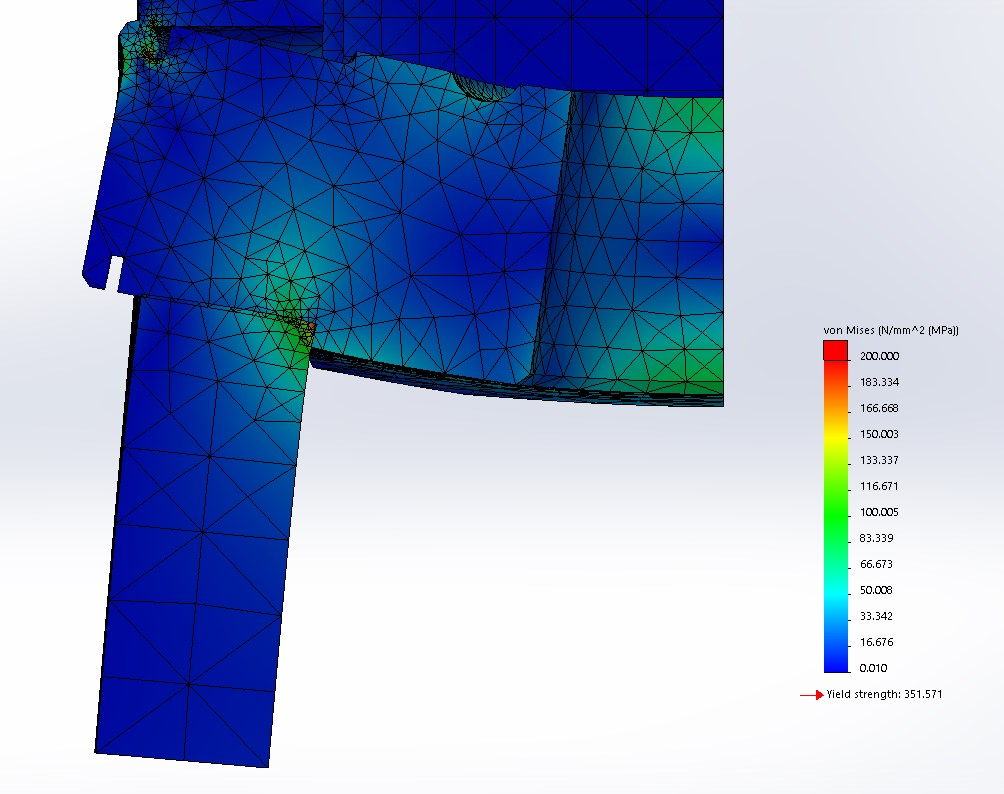
\includegraphics[width=.5\textwidth]{imgs/fem/Quarto1}
\caption{Affinamento della mesh in corrispondenza del contatto traversa-piastrone.}
\label{fig:Quarto1}
\end{figure}
\begin{figure}[H]
\centering
  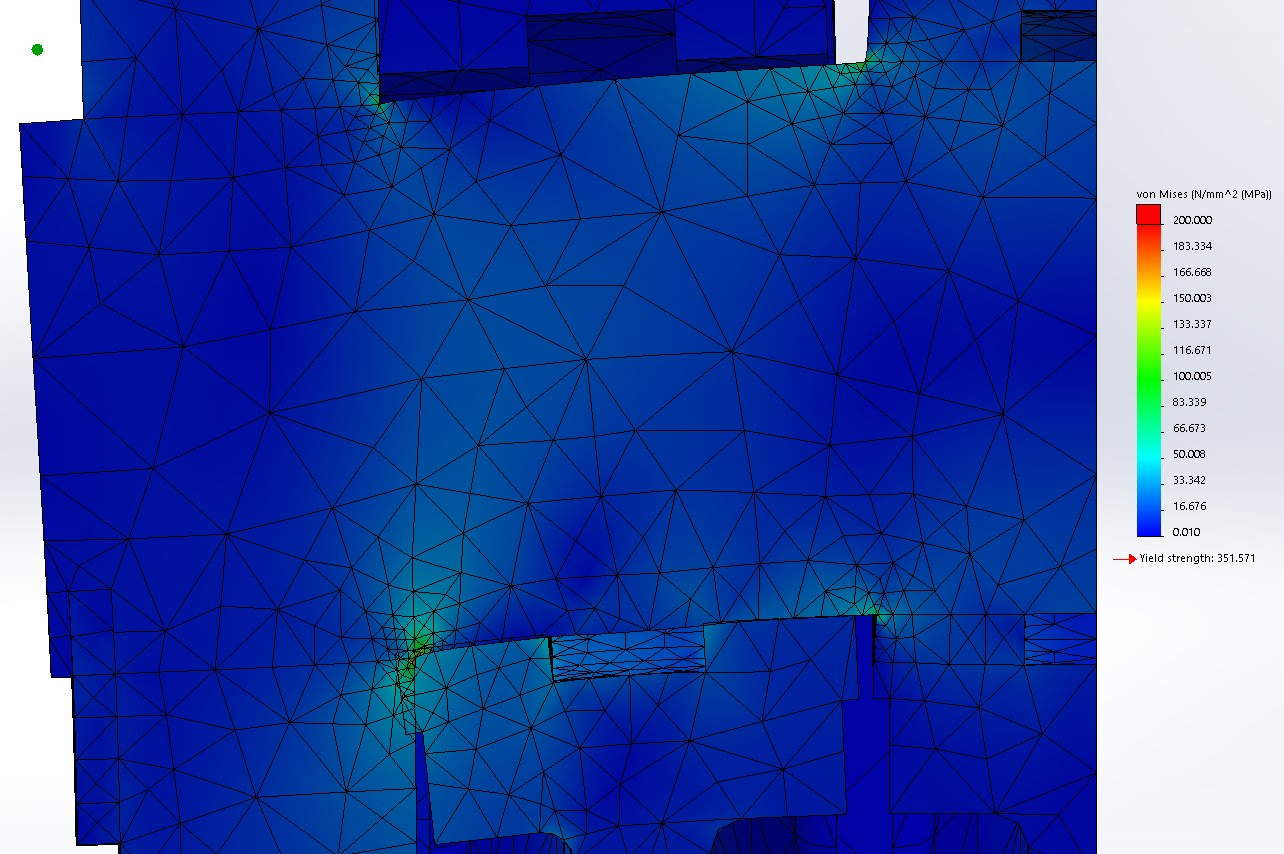
\includegraphics[width=.5\textwidth]{imgs/fem/Quarto2}
\caption{Affinamento della mesh in corrispondenza dei contatti puleggia-asse e asse-piastrone.}
\label{fig:Quarto2}
\end{figure}
\begin{figure}[H]
\centering
  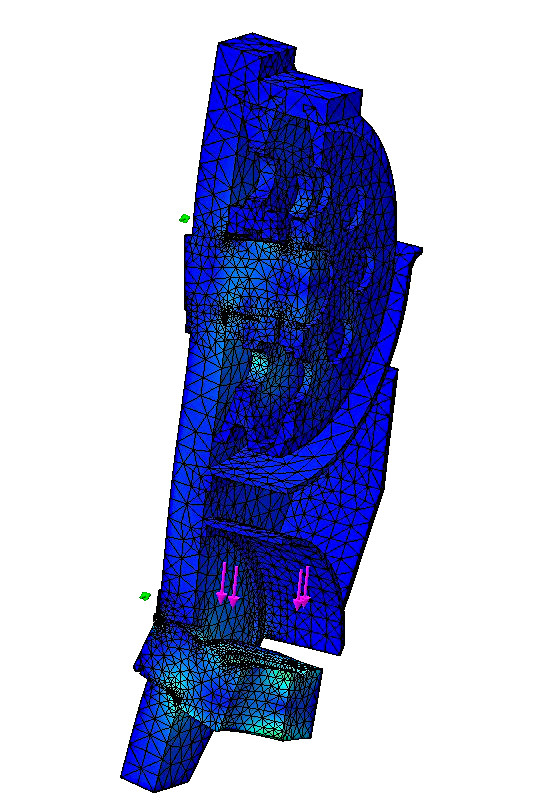
\includegraphics[width=.45\textwidth]{imgs/fem/Quarto3}
\caption{Deformata complessiva.}
\label{fig:Quarto3}
\end{figure}
Oltre al quarto di modello sono state fatte delle simulazioni su un mezzo modello semplificato. 
\begin{figure}[H]
\centering
  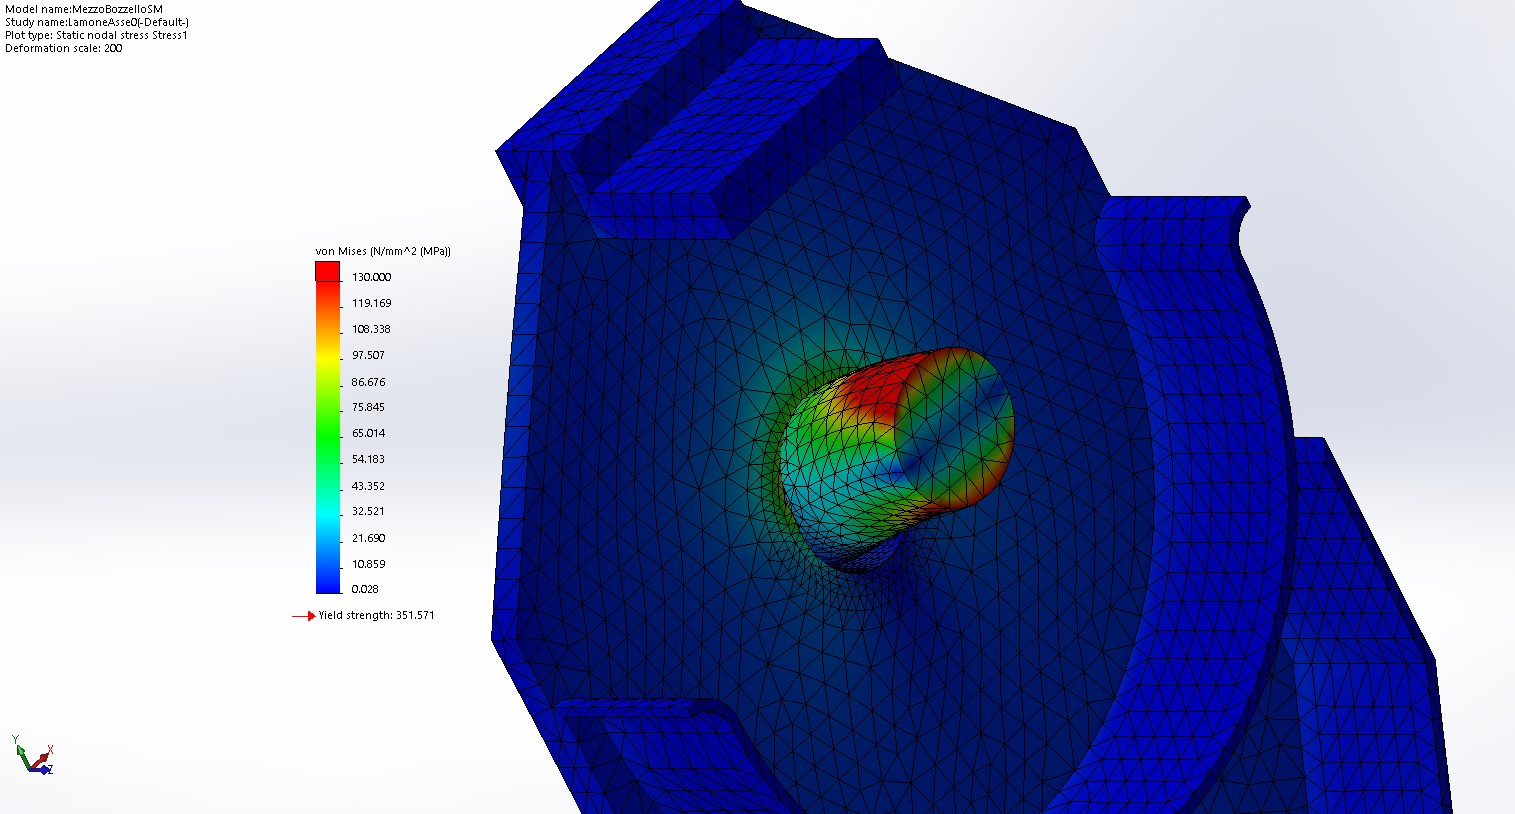
\includegraphics[width=.6\textwidth]{imgs/fem/MezzoBozzello-Asse}
\caption{}
\label{fig:MezzoBozzello-Asse}
\end{figure}
Viene infine riportata la simulazione riguardante il foro praticato sul lamone-piastrone, sede del perno della traversa; è stato applicato un carico da cuscinetto pari ala portata nominale.
\begin{figure}[H]
\centering
  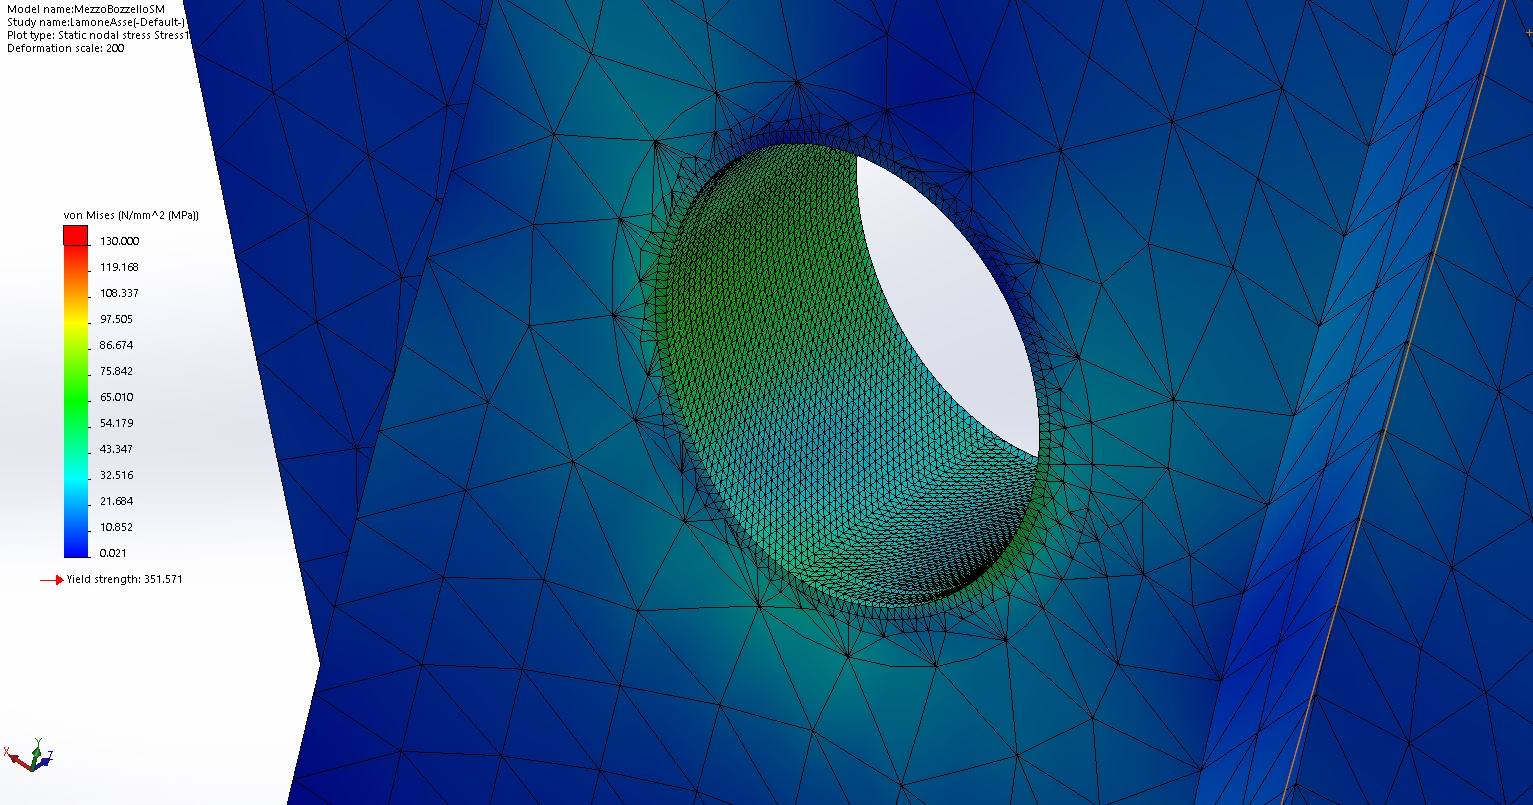
\includegraphics[width=.6\textwidth]{imgs/fem/MezzoBozzello-Traversa.jpg}
\caption{}
\label{fig:MezzoBozzello-Traversa}
\end{figure}
La relativa curva di convergenza viene riportata di seguito. 
\begin{figure}[H]
\centering
  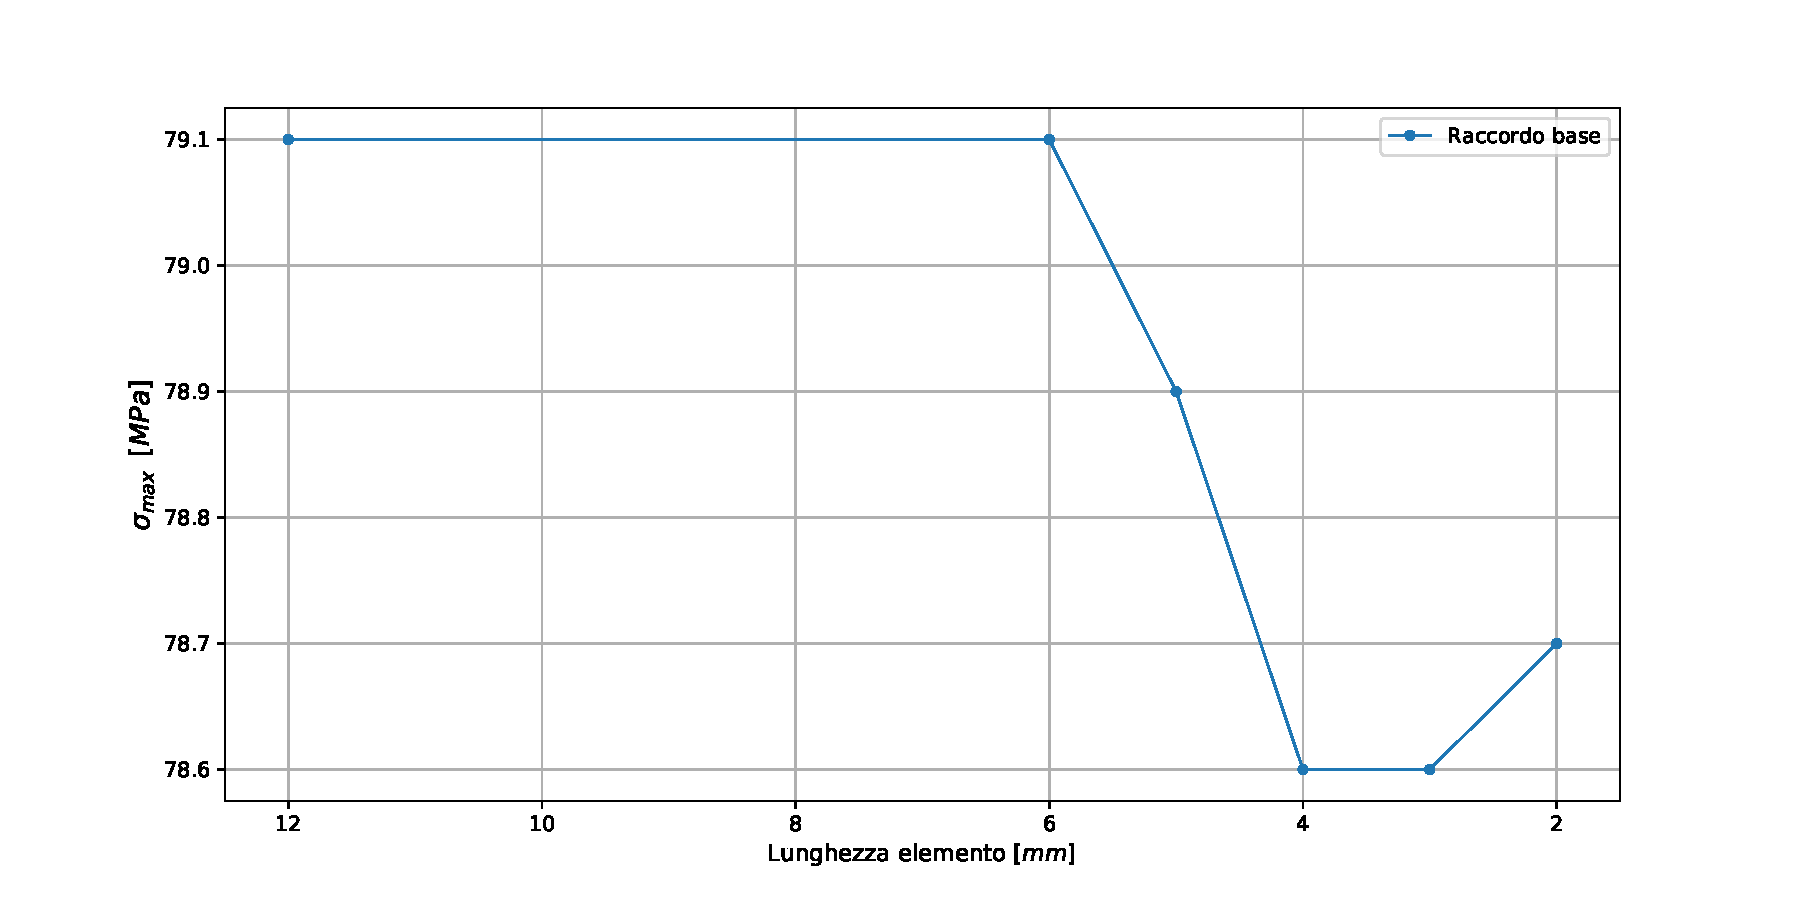
\includegraphics[width=.55\textwidth]{imgs/fem/MezzoBozzello-Traversa.pdf}
\caption{}
\label{fig:MezzoBozzello-TraversaConv}
\end{figure}

\subsection{Analisi del gancio}
In questa analisi si è considerato solo il gancio, tagliando gambo e la parte finale del becco. Si considera metà modello con un vincolo di simmetria. 
Sulla sezione di sviluppo del gambo è stato invece inserito un vicolo fisso. 
Per l'applicazione del carico è stata simulata sommariamente l'applicazione della fune in direzione verticale e a $45^{\circ}$ come mostrato nelle immagini in figura \ref{fig:GancioCaricoFin}. 
\begin{figure}[H]
\centering
  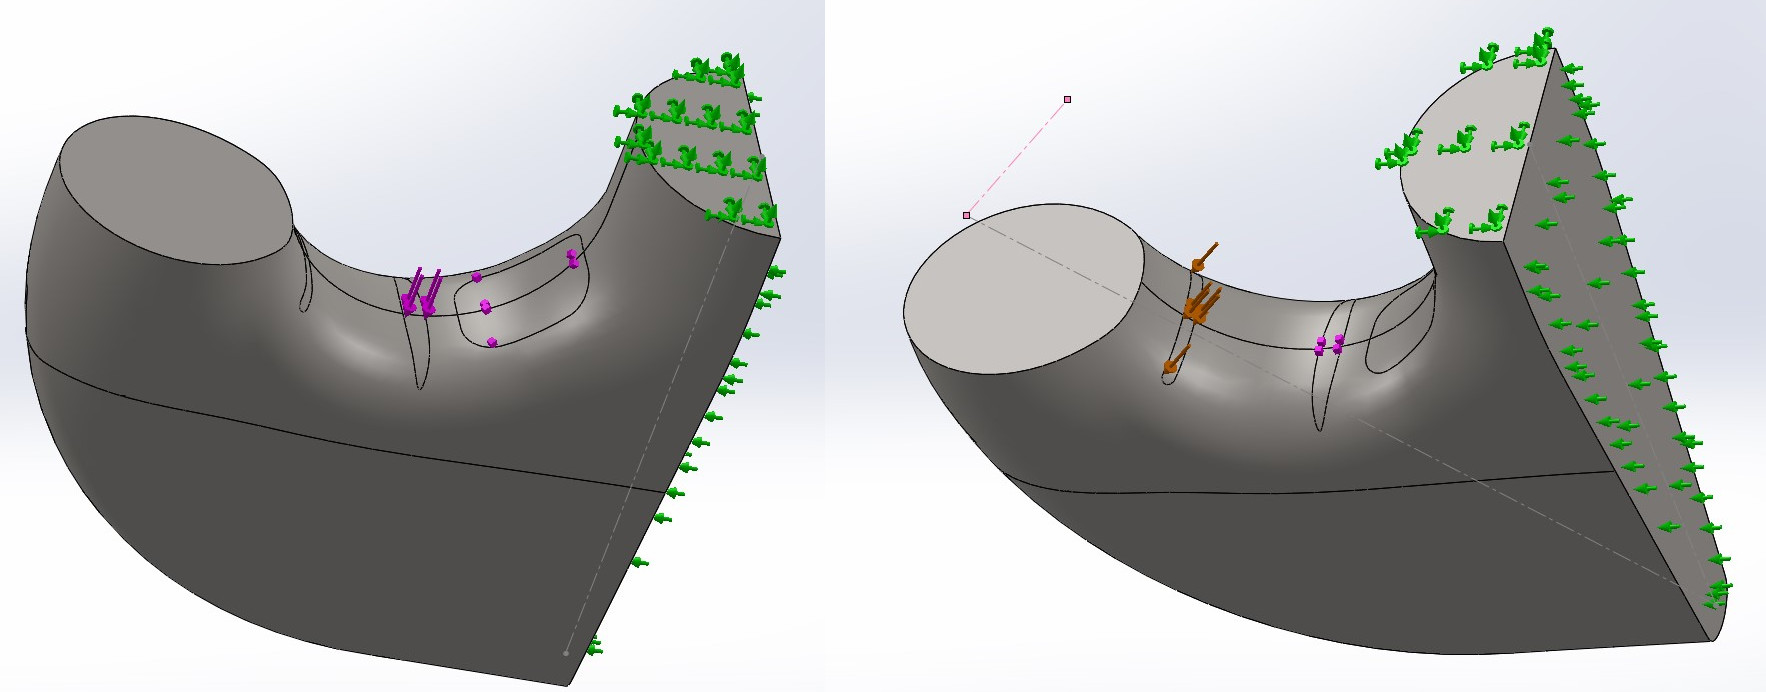
\includegraphics[width=.8\textwidth]{imgs/fem/GancioCaricoFin}
\caption{Schema di carico verticale a sinistra, a $45^{\circ}$ a destra.}
\label{fig:GancioCaricoFin}
\end{figure}
\begin{figure}[H]
\centering
  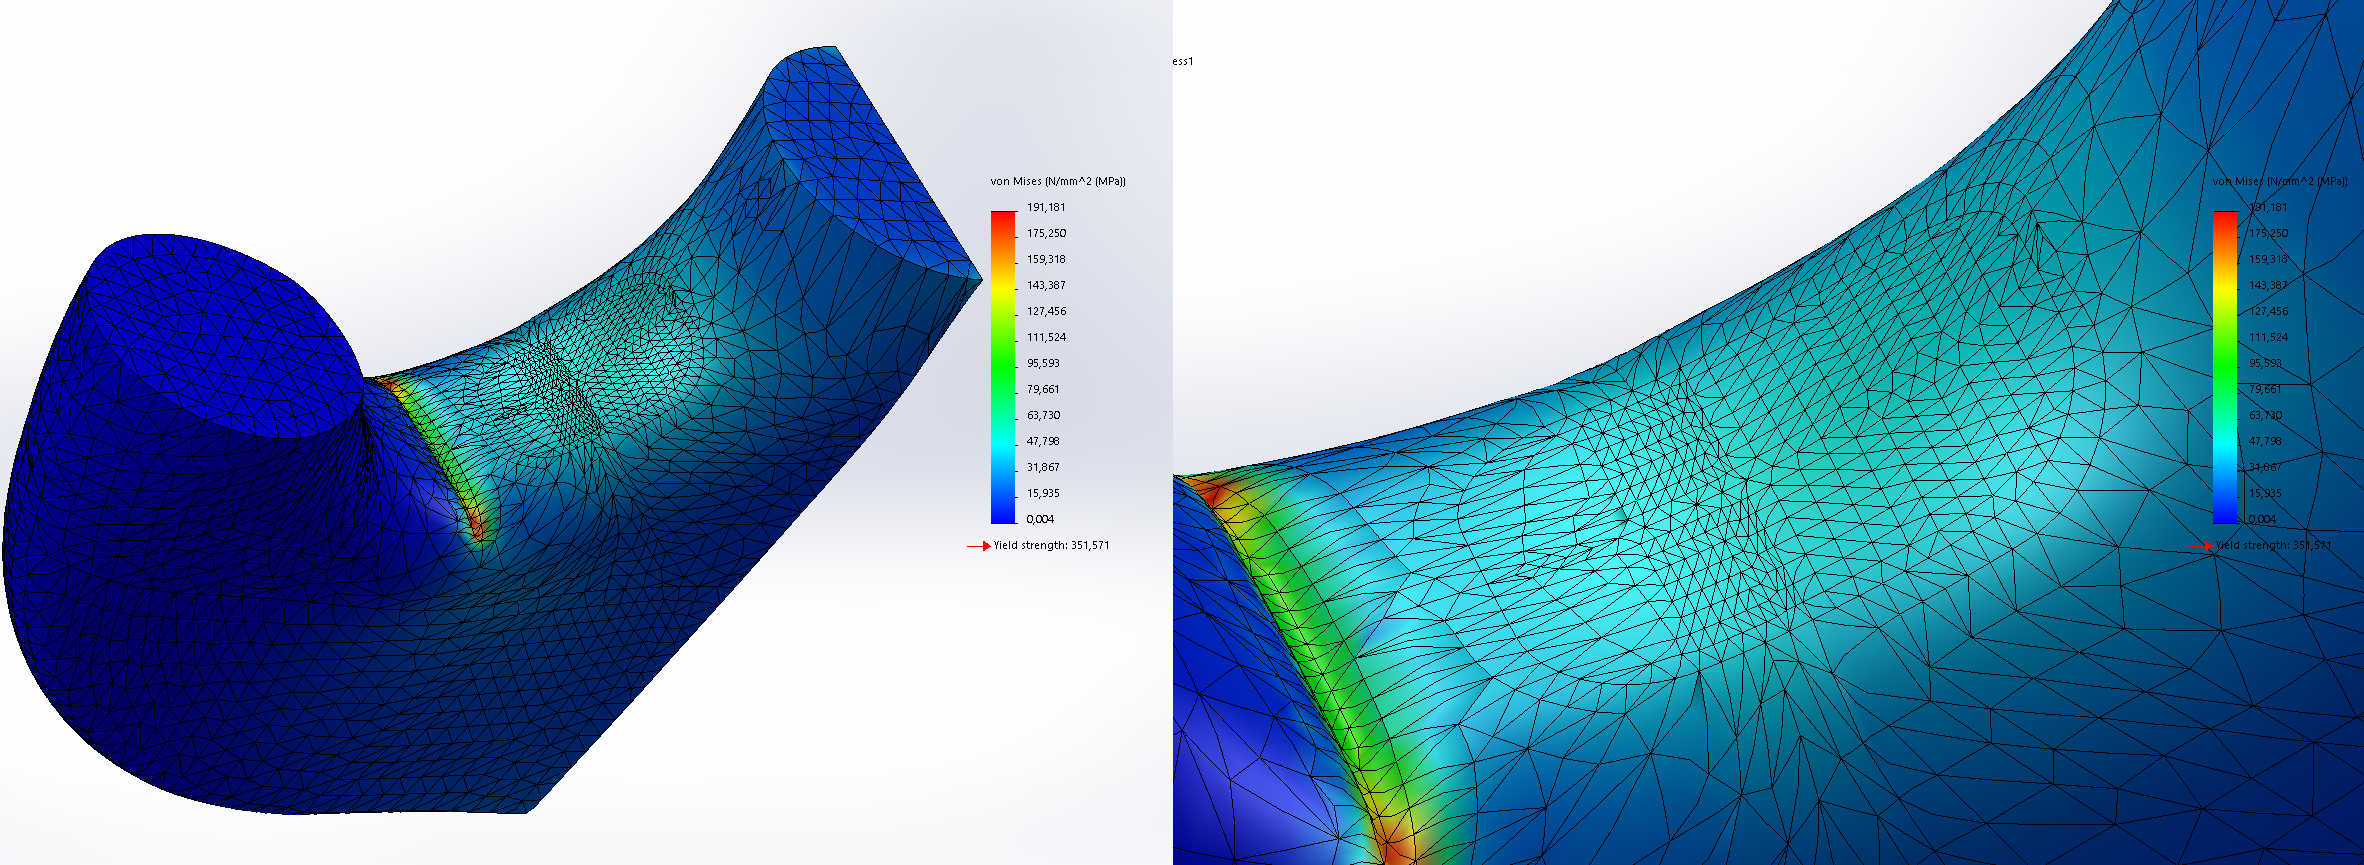
\includegraphics[width=.8\textwidth]{imgs/fem/GancioFeaFinal}
\caption{Sforzi indotti dal carico verticale.}
\label{fig:GancioFeaFinal}
\end{figure}
I risultati delle simulazioni sono andati a buon fine. 
La mesh è stata via via affinata nella zona di massima sollecitazione a trazione, in questo modo è stato possibile diagrammare i grafici di convergenza in figura \ref{fig:Gancio}. 
Per il carico posto verticalmente è stata raggiunta una sollecitazione massima di $54.7 \; MPa$ mentre per il carico posto a $45^{\circ}$ la sollecitazione massima aveva un valore di $100.3\; MPa$.
\begin{figure}[H]
\centering
  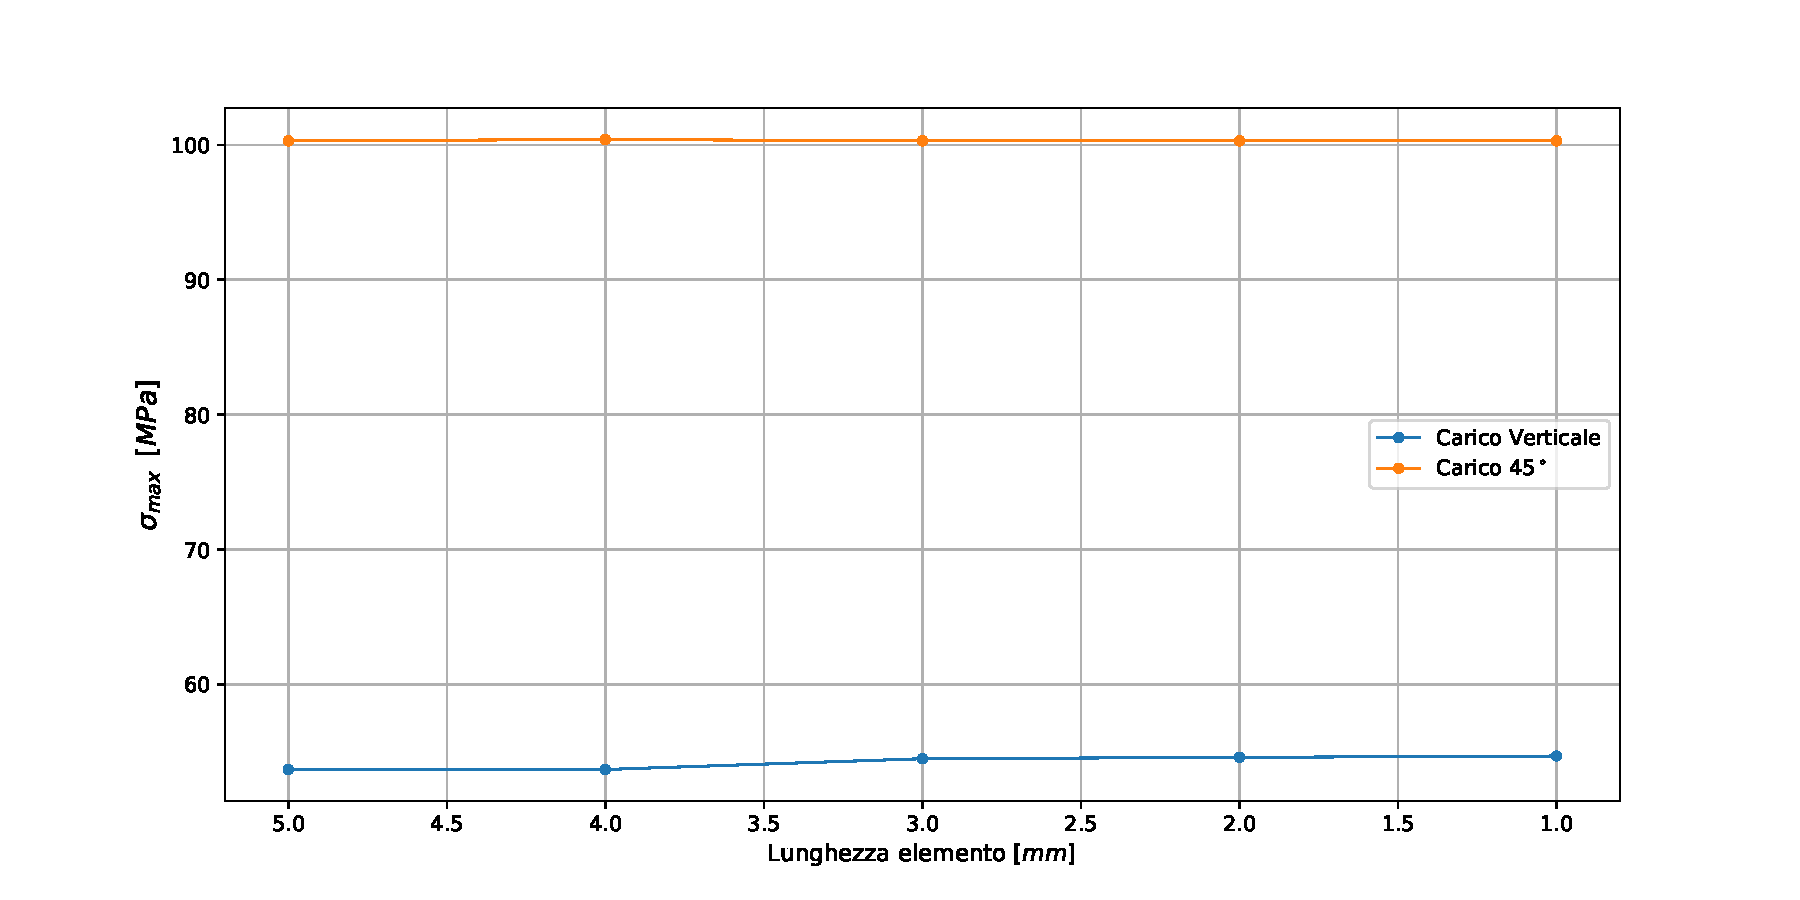
\includegraphics[width=.6\textwidth]{imgs/fem/Gancio}
\caption{Diagramma di convergenza del gancio.}
\label{fig:Gancio}
\end{figure}

\subsection{Analisi del gambo del gancio}
In questa analisi è stato rimosso il gancio e si considera solamente il gambo.
Da un'analisi grezza si è visto che i punti più sollecitati sono i due raccordi concavi.
Una prima simulazione su una mesh grezza ha permesso di individuare una criticità: il limite del vincolo fisso, posto sulla zona filettata, era decisamente troppo vicino al raccordo superiore. La discontinuità tra superficie vincolata e superficie libera fa emergere degli sforzi singolari (non reali), questo campo di sforzi va a sovrapporsi al campo di sforzi reale andando ad invalidare la simulazione. 
Per evitare questo problema si è allontanata la linea di discontinuità dal raccordo in questione andando a diminuire la superficie vincolata. 
Si è quindi proceduto al raffinamento della mesh nei raccordi maggiormente sollecitati per valutare la convergenza. 
\begin{figure}[H]
\centering
  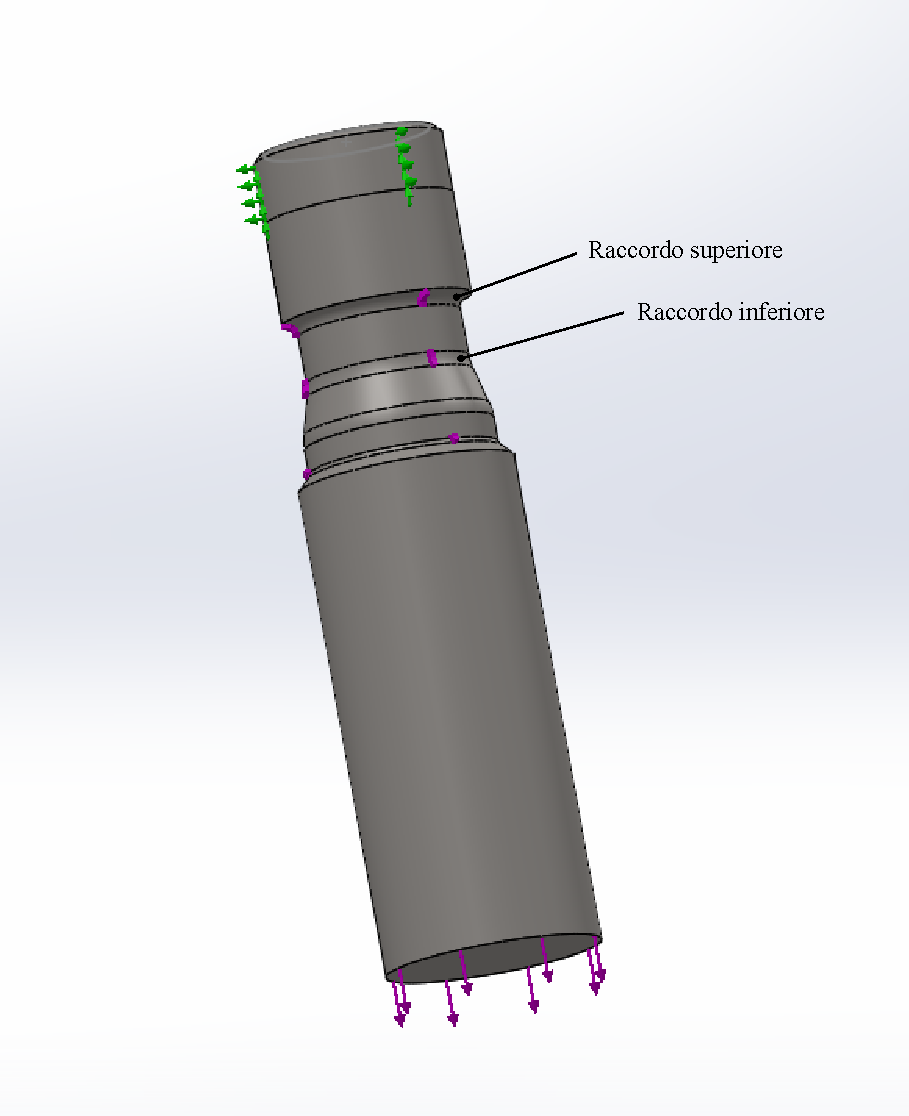
\includegraphics[width=.4\textwidth]{imgs/fem/SimGambo2.pdf}
\caption{Carico e vincoli del gambo del gancio.}
\label{fig:SimGambo2}
\end{figure}
\begin{figure}[H]
\centering
  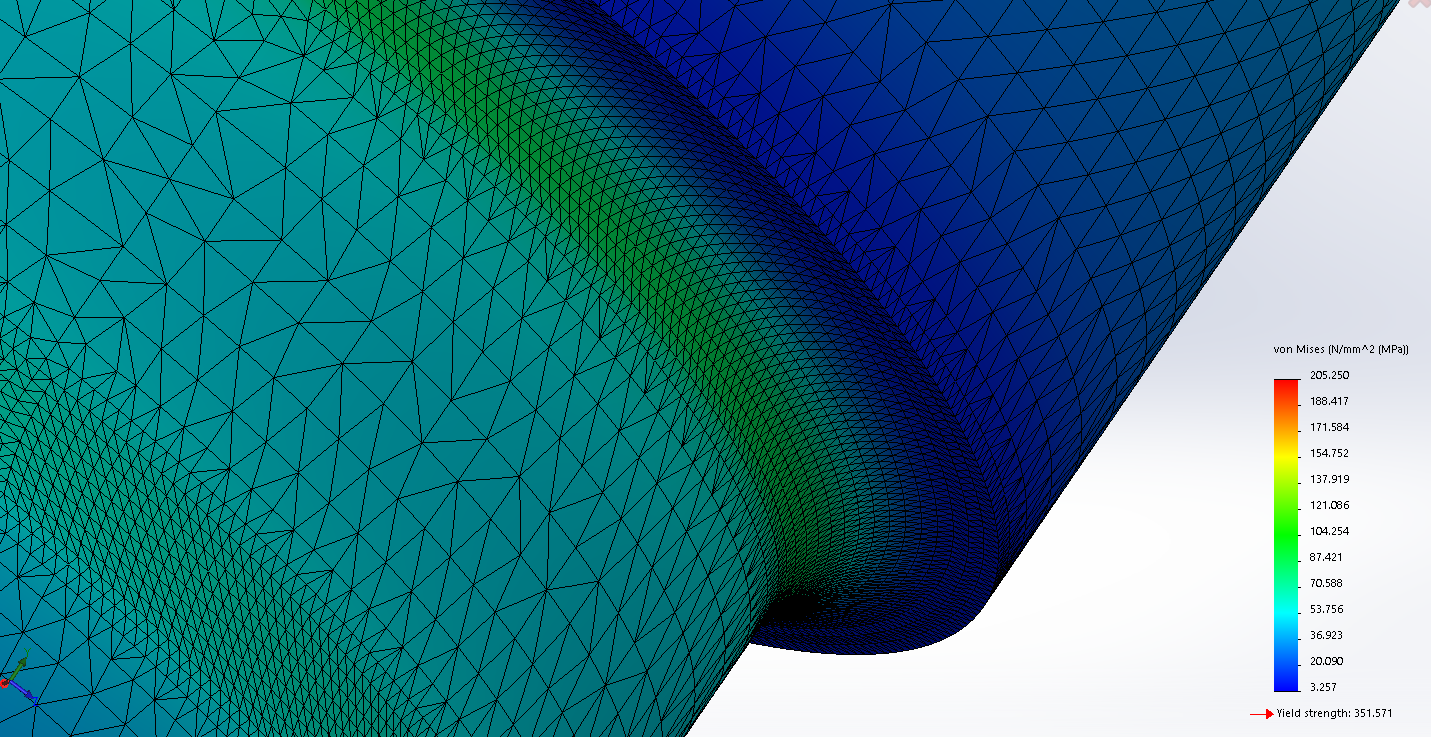
\includegraphics[width=.7\textwidth]{imgs/fem/SimGambo1}
\caption{Raccordi maggiormente sollecitati.}
\label{fig:SimGambo1}
\end{figure}
Di seguito sono riportati i diagrammi di convergenza per i due raccordi più sollecitati. 
I valori di sollecitazione sono entro i limiti, viene calcolato uno sforzo massimo di $86.9\;MPa$ per il raccordo superiore mentre un valore di $75.6\;MPa$ per quello inferiore. 
\begin{figure}[H]
\centering
  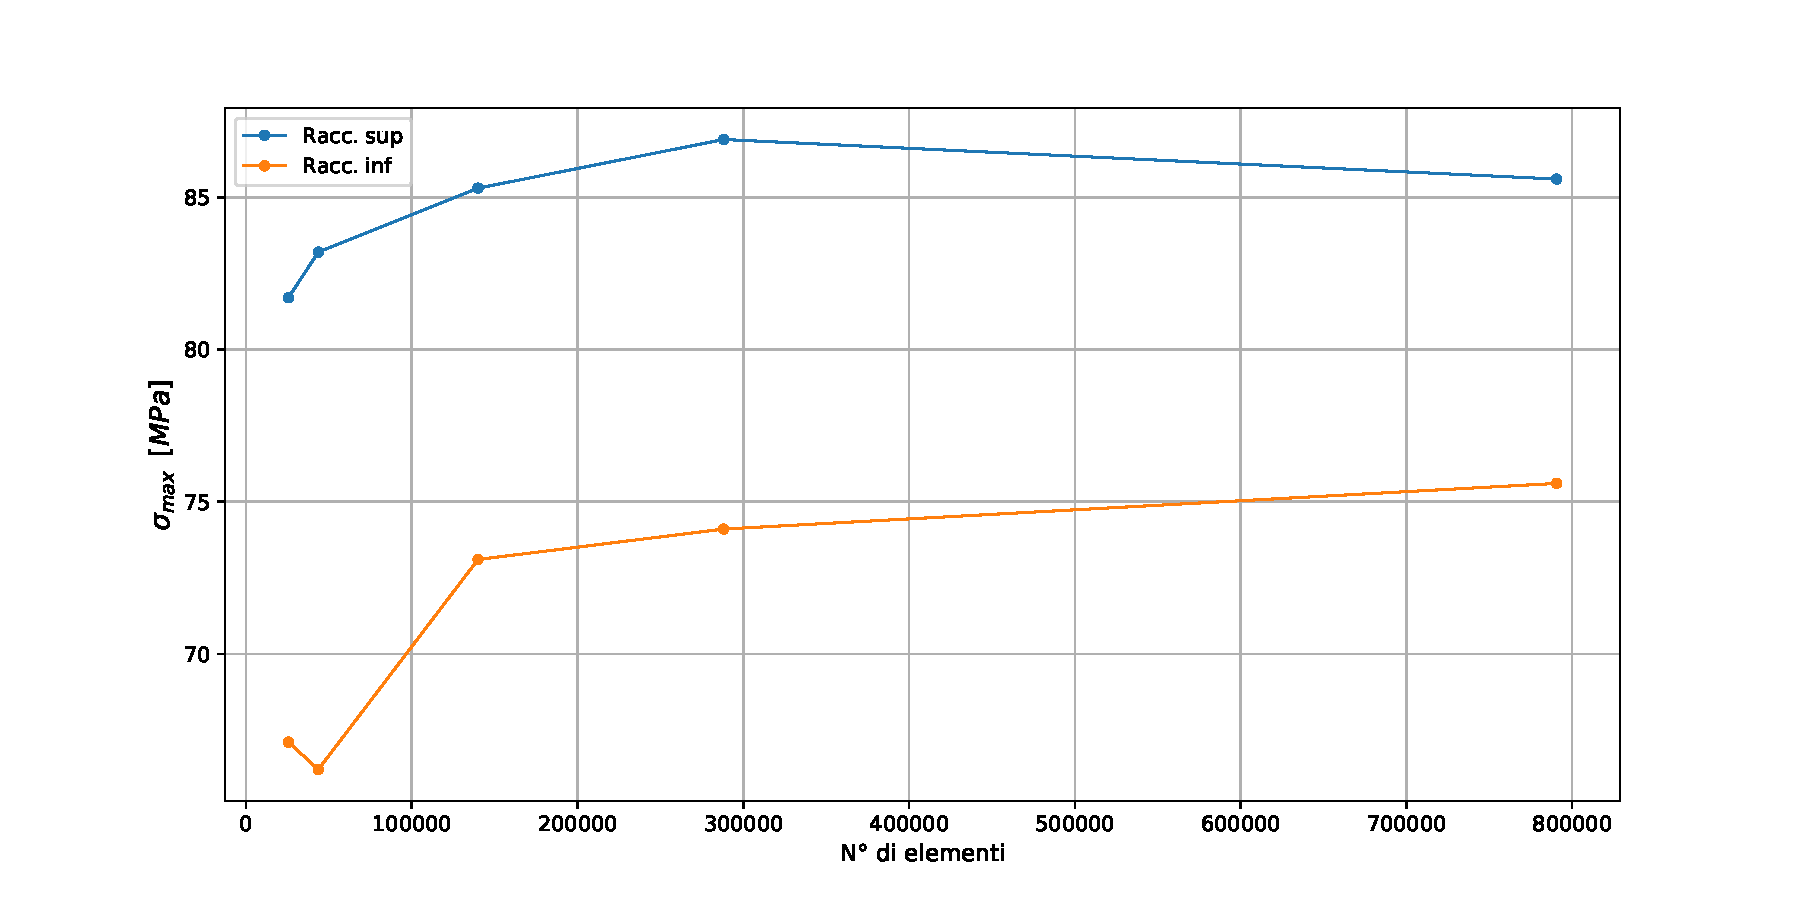
\includegraphics[width=.6\textwidth]{imgs/fem/GamboGancioConv}
\caption{Diagramma di convergenza del gambo del gancio.}
\label{fig:GamboGancioConv}
\end{figure}

\subsection{Analisi della traversa}
Anche per lo studio della traversa si è semplificato il modello andando a rimuovere dado e sfere. Lo studio è stato effettuato solamente su metà modello, imponendo un vincolo di simmetria.
Il calcolo viene applicato uniformemente sulla pista di rotolamento delle sfere, questo sarà pari a metà della portata nominale.
La parte inferiore del perno è stata infine vincolata con vincolo fisso. 

\begin{figure}[H]
\centering
  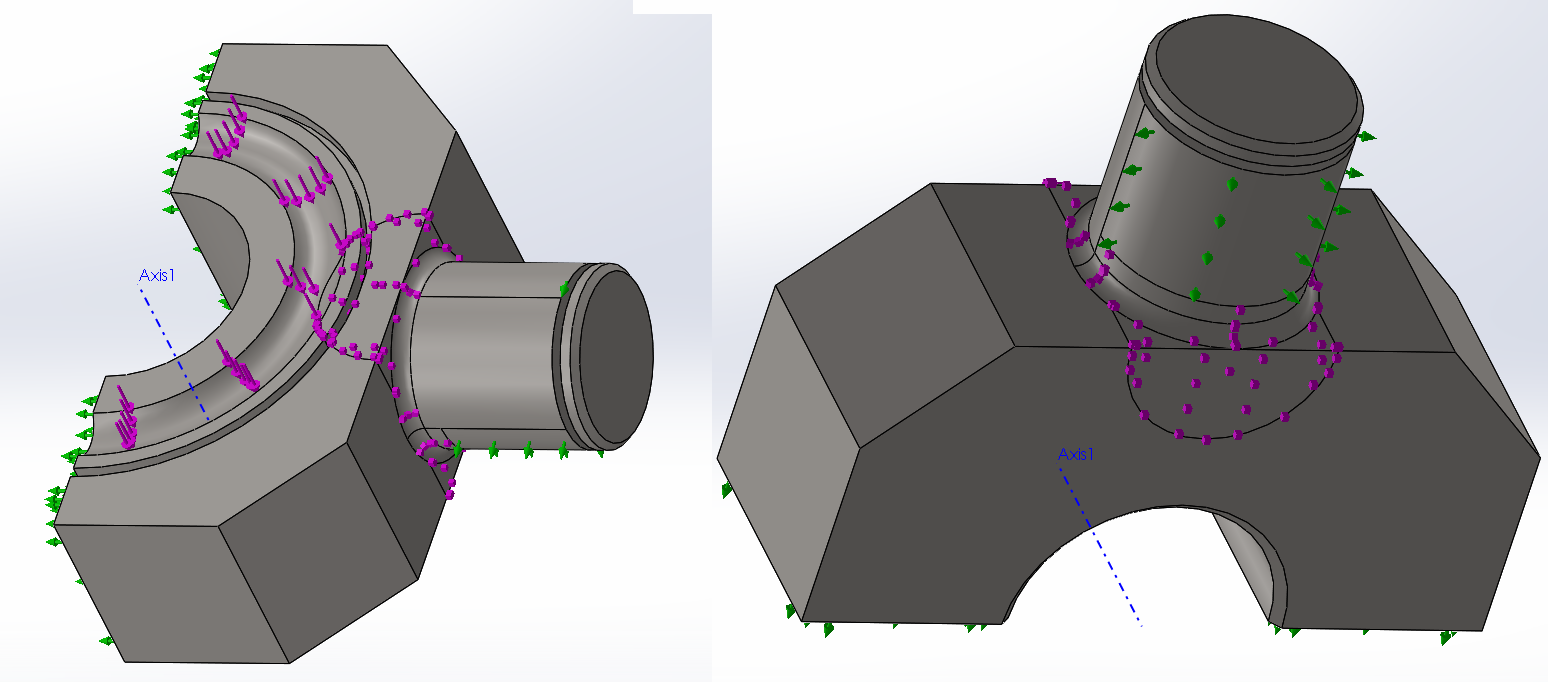
\includegraphics[width=.8\textwidth]{imgs/fem/SimTraversaCarico}
\caption{Si può vedere chiaramente in rosso la zona in cui sono presenti gli sforzi singolari.}
\label{fig:GamboGancioConv}
\end{figure}
Domo una simulazione su mesh grezza è stato verificato che il punto maggiormente sollecitato, come previsto, è situato sulla parte inferiore del raccordo del perno. 
In questo punto gli sforzi salcolati superavano i limiti imposti. 
Per questo motivo sono state modificale le quote della traversa, l'altezza $H_t$ è stata portata da un valore di $113 \; mm$ ad un valore di $130 \; mm$ in questo modo è stato possibile aumentare anche i diametri del perno e di conseguenza aumentare la sezione resistente dello stesso. 
In fase di modellazione è stato inoltre necessario aumentare il diametro della pista di rotolamento per permettere l'inserimento delle 22 sfere. 
Questa modifica ha comportato un maggior distanziamento dei piastroni, un aumento della lunghezza dell'asse e di conseguenza un aumento dell'ingombro delle carrucole (quota $T$). Il gioco assiale complessivo è stato aggiornato a $8\;mm$.

\begin{figure}[H]
\centering
\begin{minipage}{.5\textwidth}
  \centering
  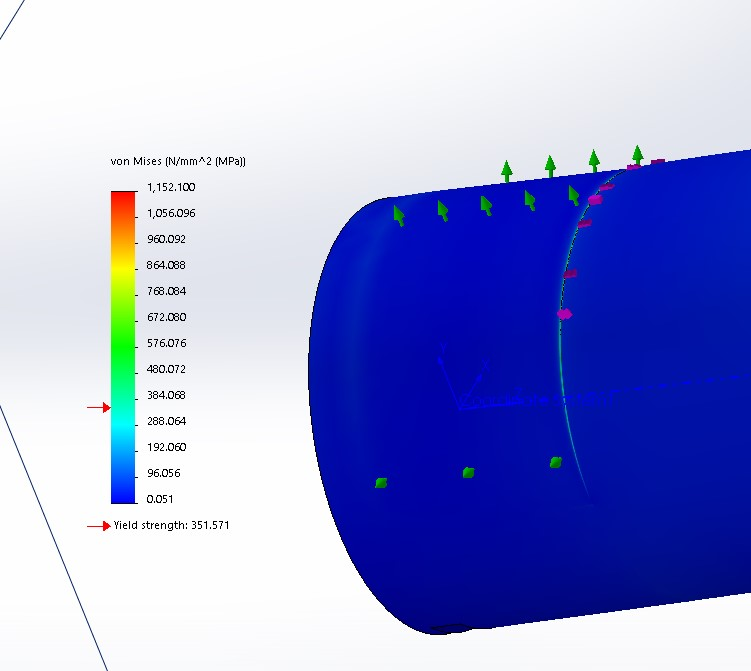
\includegraphics[width=.9\linewidth]{imgs/fem/AsseSim1}
  \captionof{figure}{}
  \label{fig:AsseSim1}
\end{minipage}%
\begin{minipage}{.5\textwidth}
  \centering
  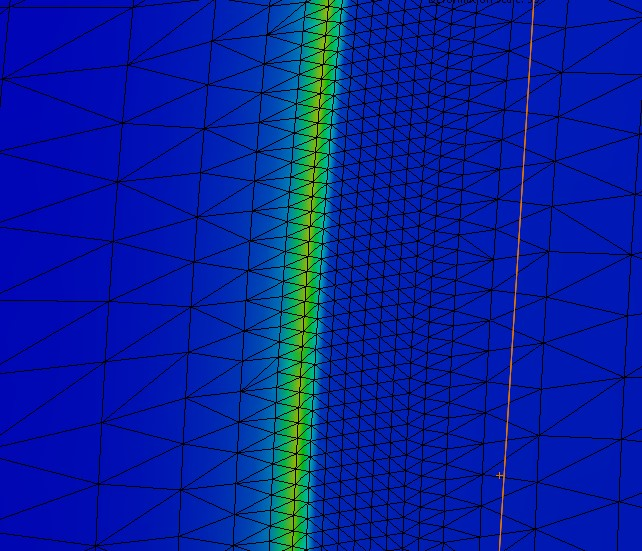
\includegraphics[width=.9\linewidth]{imgs/fem/AsseSim2}
  \captionof{figure}{}
  \label{fig:AsseSim2}
\end{minipage}
\end{figure}

\begin{figure}[H]
\centering
  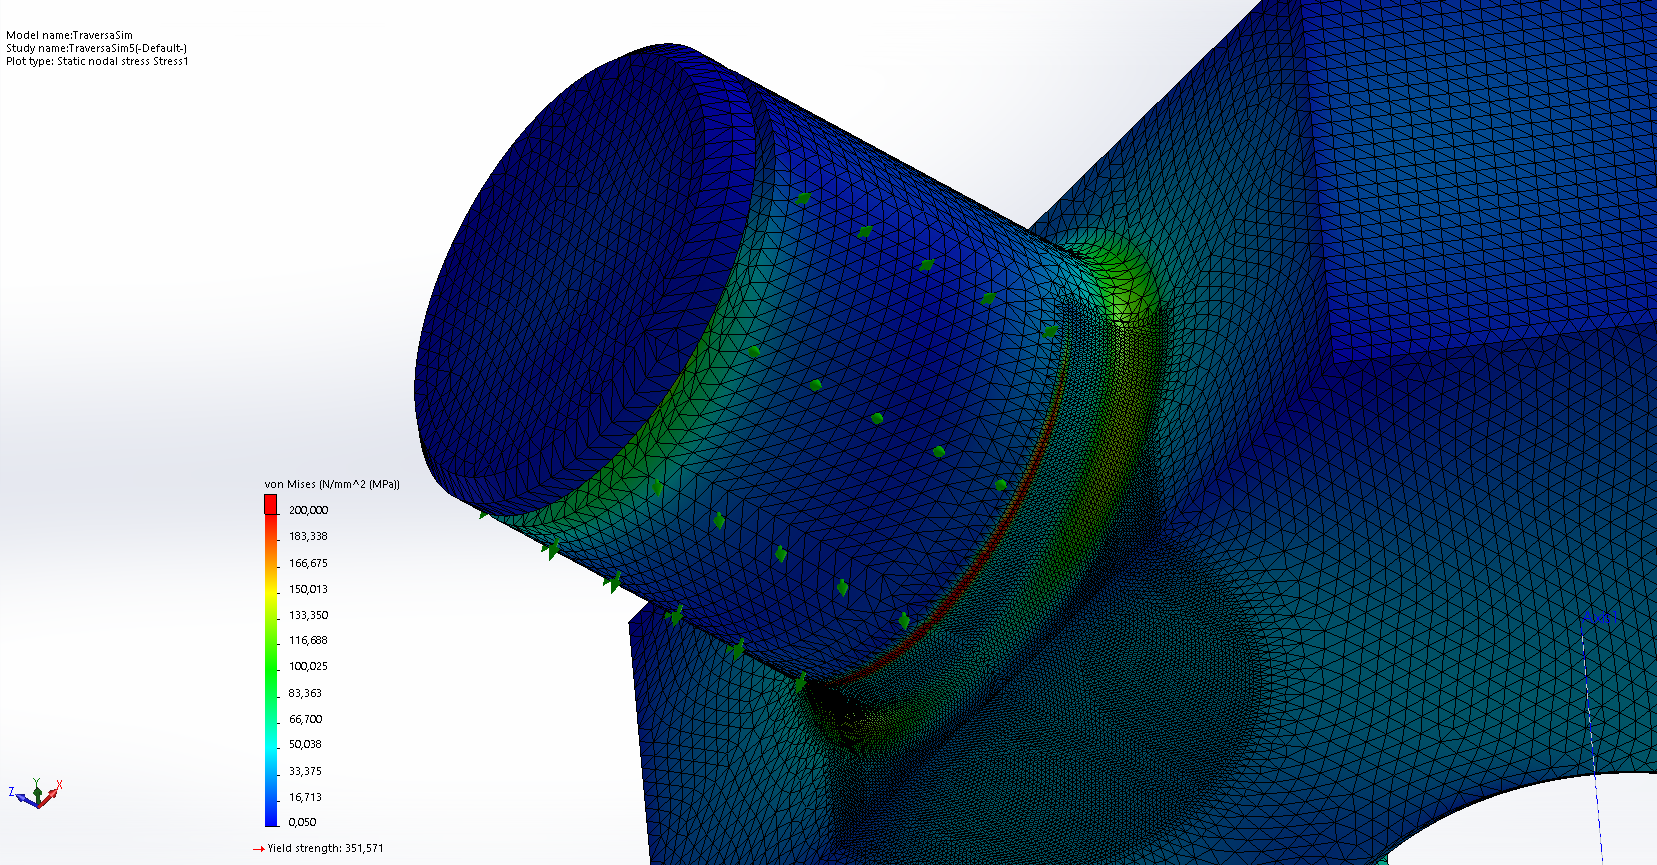
\includegraphics[width=.7\textwidth]{imgs/fem/TraversaSim1}
\caption{}
\label{fig:GamboGancioConv}
\end{figure}
Anche in questo caso, a causa della sollecitazione singolare in vicinanza del raccordo del perno, si è deciso di diminuire la superficie vicolata in modo da allontanare la discontinuità dal punto di interesse.
\begin{figure}[H]
\centering
  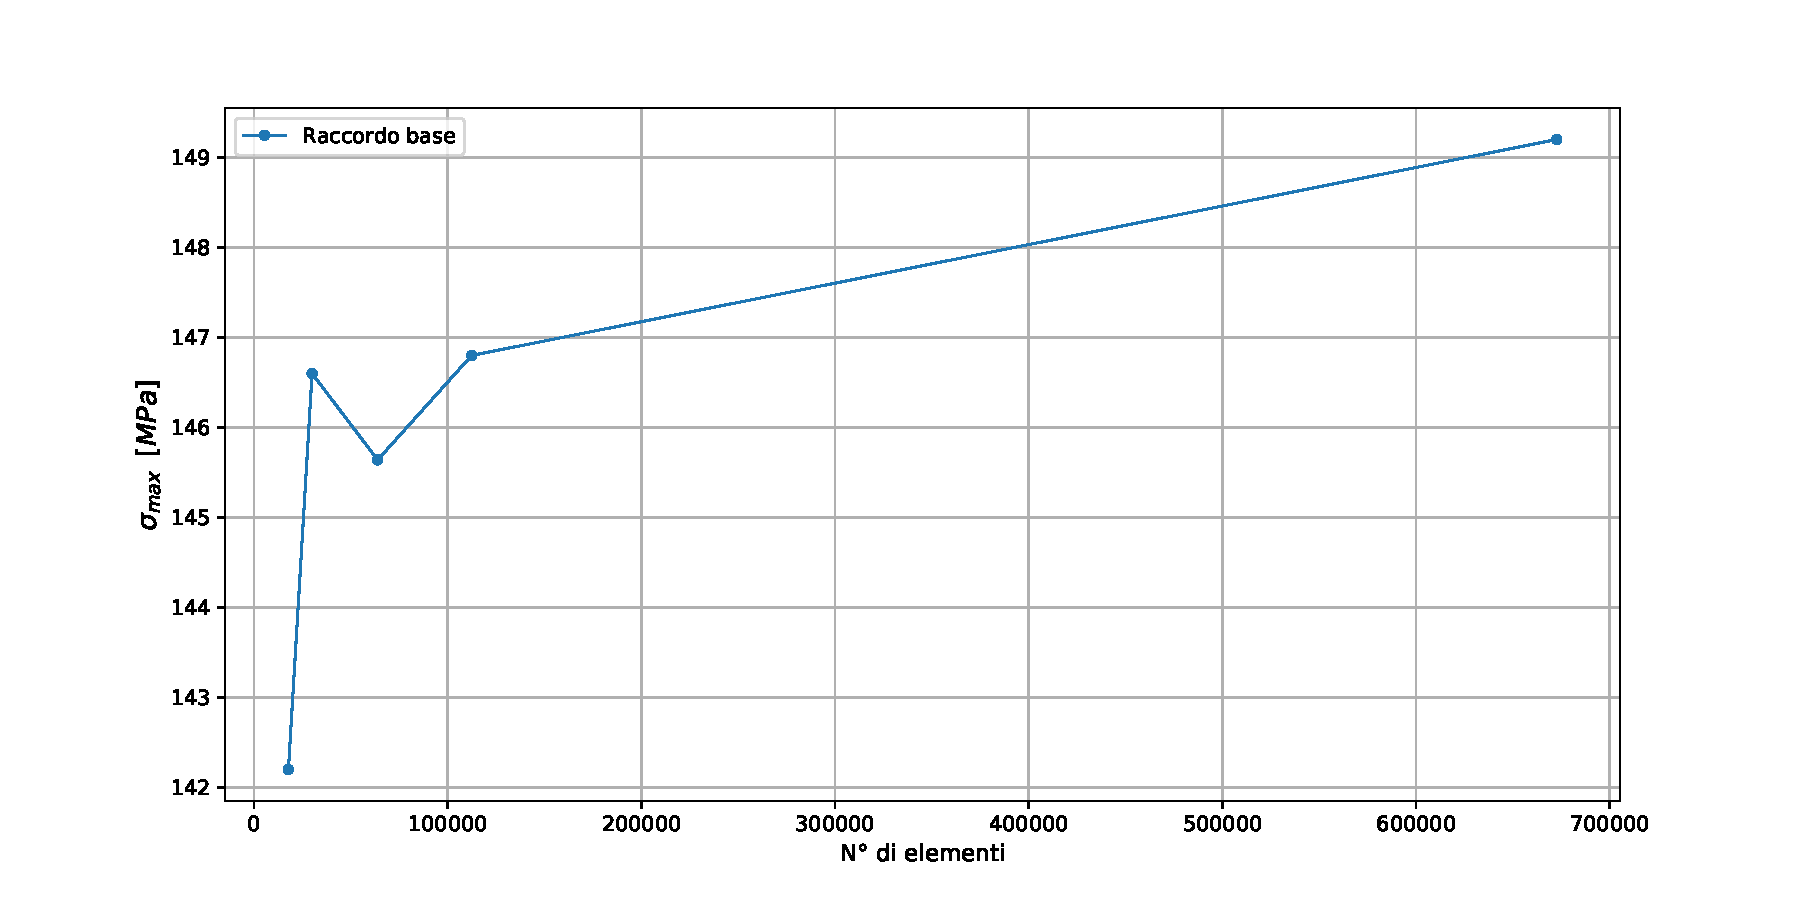
\includegraphics[width=.6\textwidth]{imgs/fem/TraversaConv}
\caption{Diagramma di convergenza della traversa.}
\label{fig:GamboGancioConv}
\end{figure}
La sollecitazione massima calcolata è di $149.2 \; MPa$.
\subsection{Analisi dell'asse}
Si procede ora con l'analisi dell'asse delle carrucole. Sono state utilizzate delle linee di divisione per individuare le superfici di contatto con le boccole.
In questo modo è stato possibile, in tali superfici, inserire un carico da cuscinetto pari alla portata nominale di dimensionamento. In corrispondenza delle superfici di contatto con i lamoni-piastroni sono stati inseriti dei vincoli di movimento radiale.
Per vincolare anche il grado di libertà di rotazione è stato posto un vincolo di rotazione su un punto del contorno esterno dell'asse.
La disposizione di vincoli e carichi è mostrata in figura \ref{fig:AsseCarico}.
\begin{figure}[H]
\centering
  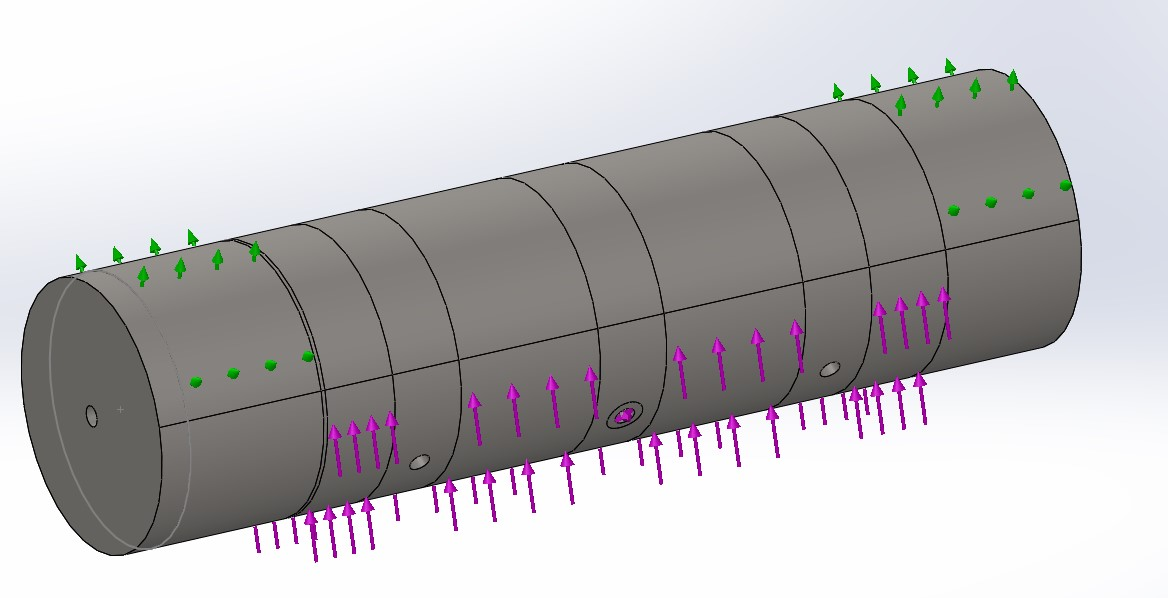
\includegraphics[width=.65\textwidth]{imgs/fem/AsseCarico}
\caption{Vincoli e carichi applicati all'asse. L'asse dei fori è ruotato a $45^{\circ}$ rispetto alla direzione della forza.}
\label{fig:AsseCarico}
\end{figure}
Dopo la simulazione sulla mesh grezza è possibile notare che in corrispondenza della discontinuità dei vincoli di movimento radiale è presente una zona notevolmente sollecitata. Affinando la mesh si può notare che tale zona di sollecitazione si restringe sempre di più e rimane confinata agli elementi finiti in corrispondenza della discontinuità di vincolo, andando via via a ridursi fino a scomparire.
Si può quindi affermare che si tratti di una sollecitazione singolare, l'infittimento della mesh funge da filtro per il campo di sollecitazioni fittizio che viene a crearsi in questa zona. 
\begin{figure}[H]
\centering
  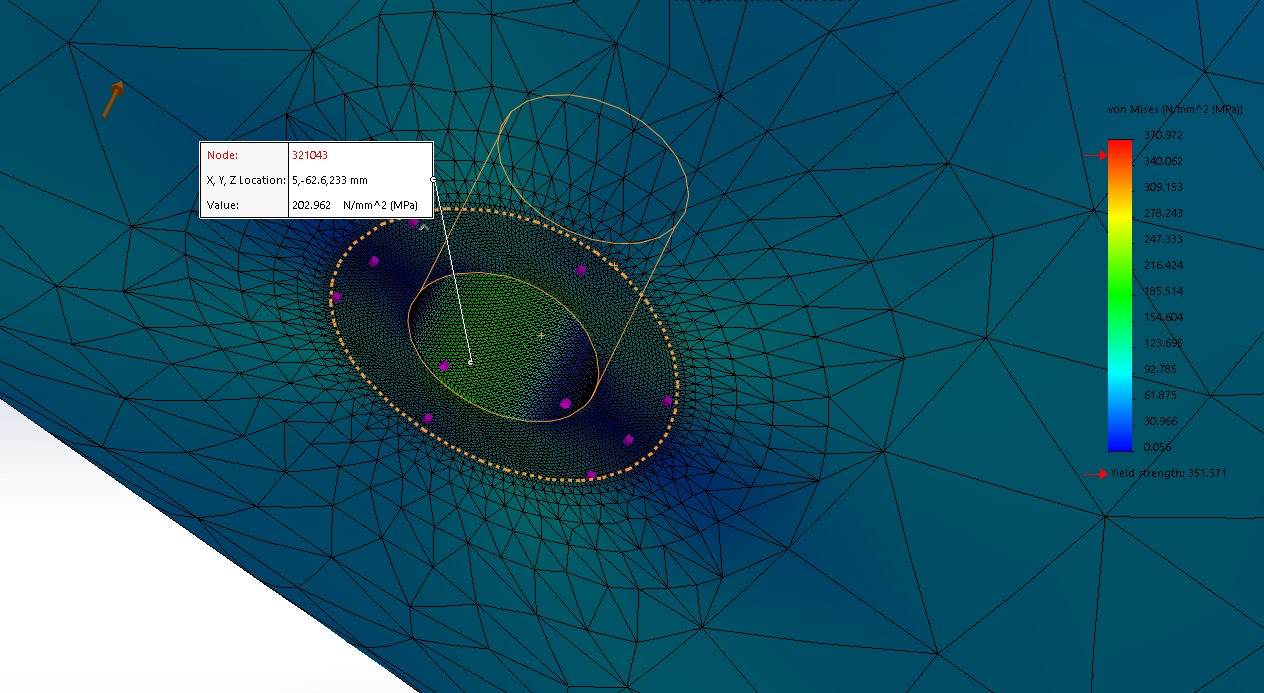
\includegraphics[width=.65\textwidth]{imgs/fem/AsseSim3}
\caption{L'immagine è riferita alla simulazione con foro avente asse verticale.}
\label{fig:AsseSim3}
\end{figure}
I valori più alti di sollecitazione si rilevano, come previsto, in corrispondenza dei fori ciechi di adduzione del grasso. Tramite linee di divisione è stata individuata una superficie in corrispondenza del foro centrale, su cui si andrà ad infittire la mesh. 
Il foro centrale è situato nel punto maggiormente sollecitato a flessione, l'effetto intaglio è  poi responsabile di un ulteriore incremento di sforzo. 
Per diminuire la sollecitazione che si genera in questo punto si può ruotare l'asse, disponendo l'asse dei fori a $45^{\circ}$ rispetto alla direzione della forza applicata. 
In questo modo si allontanano i fori dalla zona di massima sollecitazione a flessione. In figura \ref{fig:Asse} sono riportati i diagrammi di convergenza delle due casistiche considerate.
Si registra una sollecitazione massima di $203 \; MPa$ nel primo caso e di $163.5 \; MPa$ per fori posti a $45^{\circ}$.
\begin{figure}[H]
\centering
  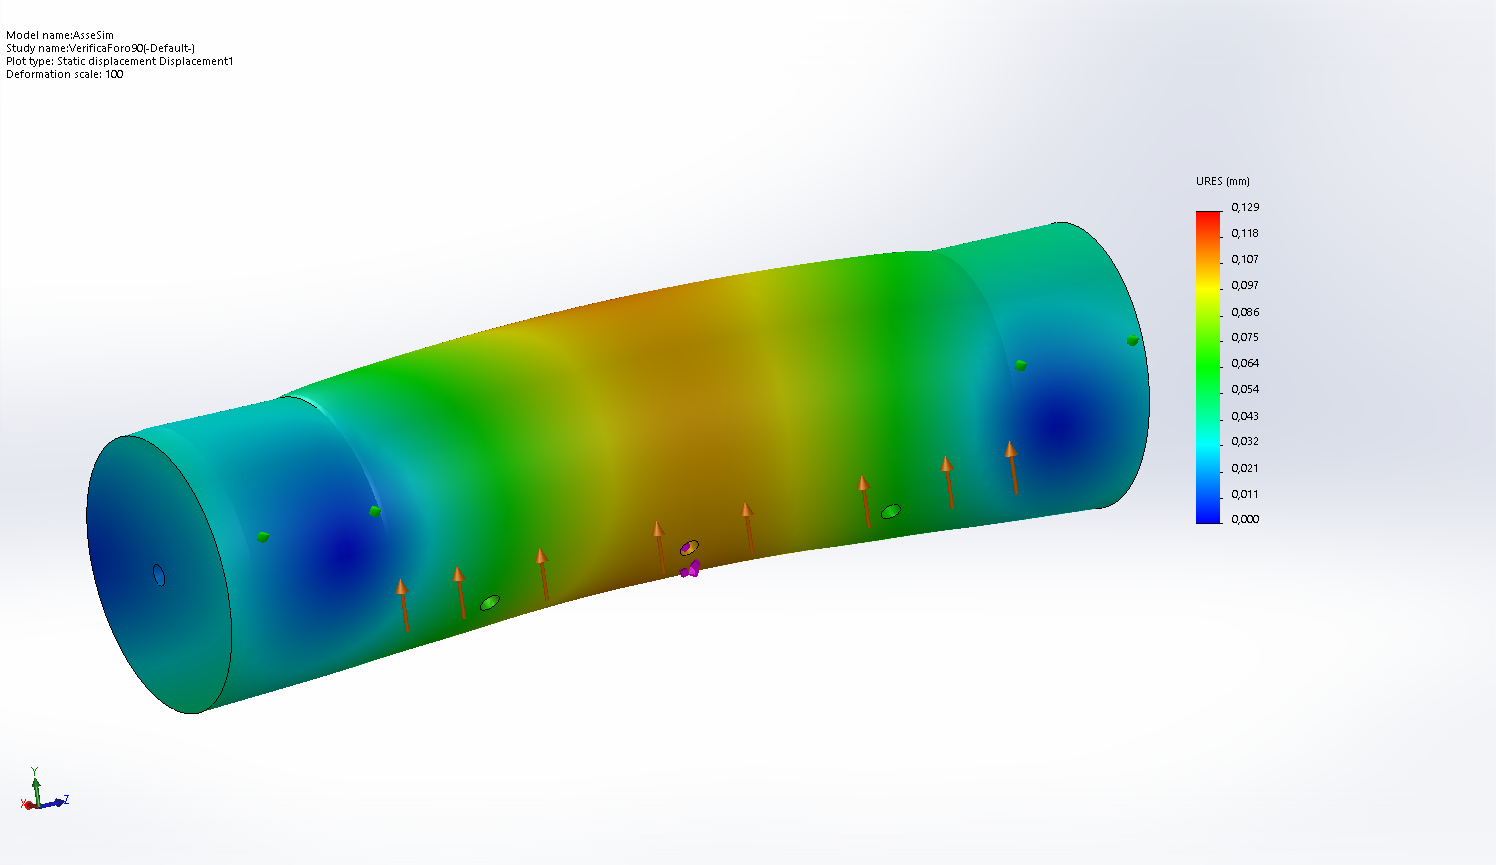
\includegraphics[width=.65\textwidth]{imgs/fem/AsseDisp}
\caption{}
\label{fig:AsseDisp}
\end{figure}
In ultimo si analizza la deformata dell'asse, i valori sono molto contenuti e si considerano ampiamente accettabili. 
\begin{figure}[H]
\centering
  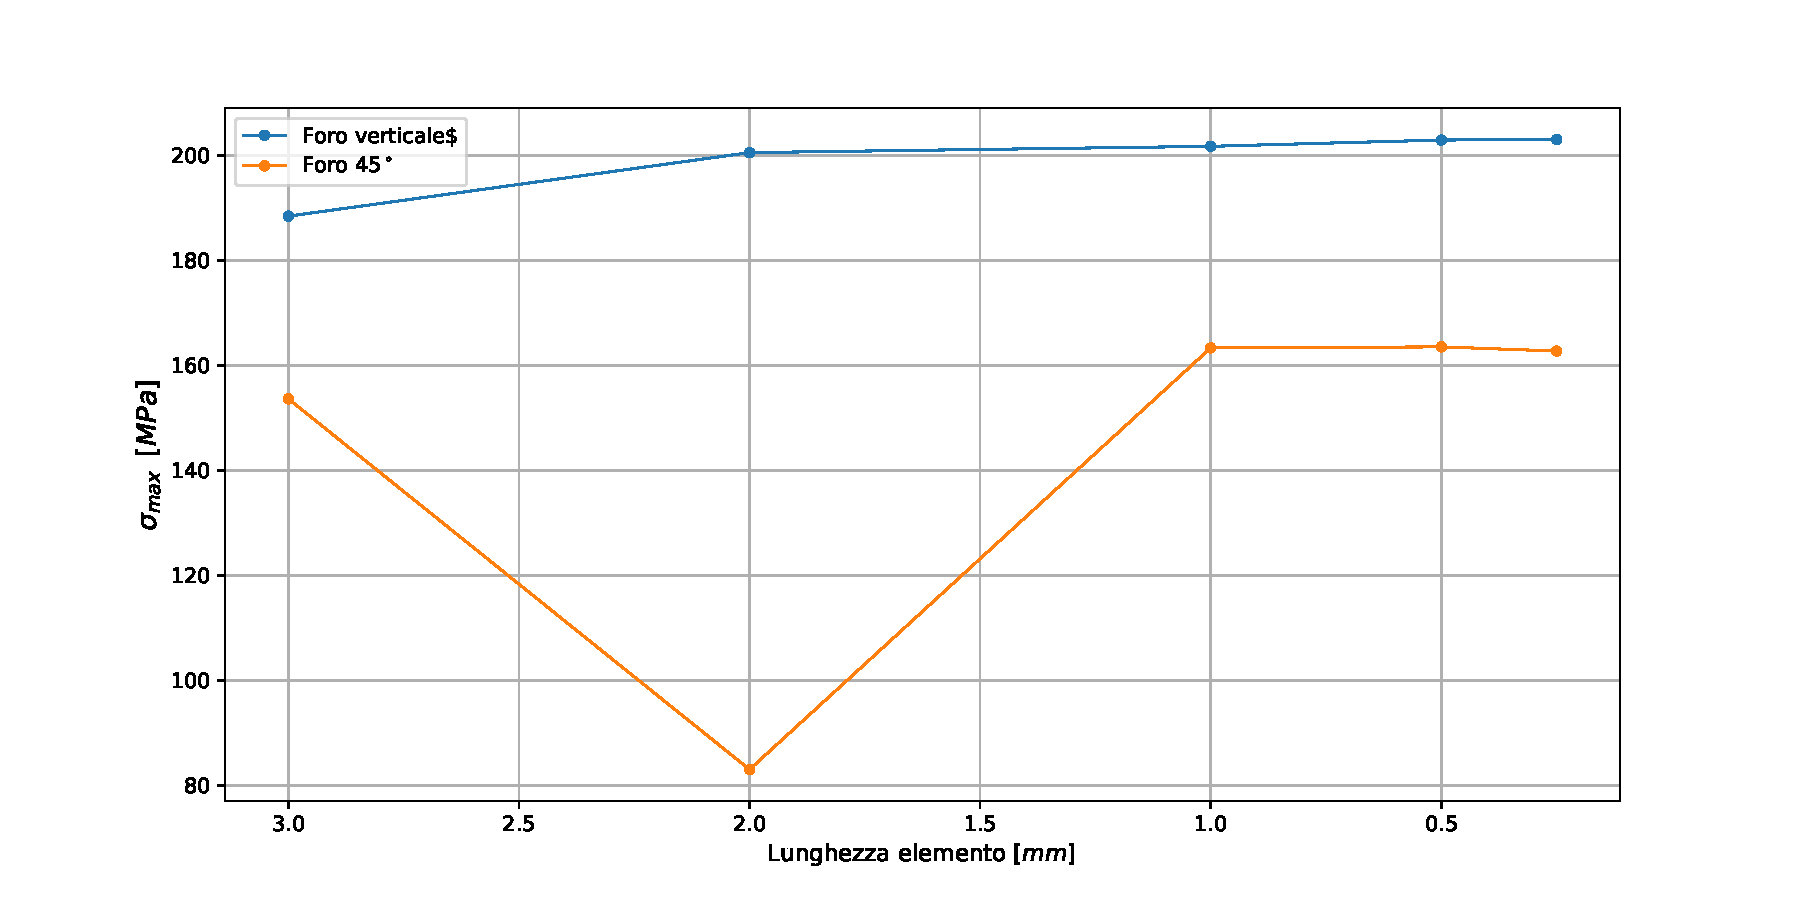
\includegraphics[width=.65\textwidth]{imgs/fem/Asse}
\caption{}
\label{fig:Asse}
\end{figure}